%%%%%%%%%%%%%%%%%%%%%%%%%%%%%%%%%%%%%%%%%%%%%%%%%%%%%%%%%%%%%%%%%%%%%%%%%%%%%%%%%%%%%%%%%%%%%%%%%%%%%%%%%%%%%%%%%%%%%%%%%%%%%%%%%%%%%%%%%%%%
%%%%%%%%%%%%%%%%%%%%%%%%%%%%%%%%%%%%%%%%%%%%%%%%%%%%%%%%%%%%%%%%%%%%%%%%%%%%%%%%%%%%%%%%%%%%%%%%%%%%%%%%%%%%%%%%%%%%%%%%%%%%%%%%%%%%%%%%%%%%
% Dies ist ein Kommentar, er wird bei der pdf-Erzeugung ignoriert.


% Dies ist eine LaTex-Vorlage für den Gebrauch im Physikalischen Praktikum I und ist als Hilfestellung zu verstehen, falls keine LaTex-Kenntnisse vorhanden sind. Einige nötige und nützliche Pakete sind bereits eingebunden und die Kapitel (\section) angelegt. Die Kapitel beinhalten teilweise Beispiele wie die Darstellung von Grafiken/Tabellen oder mathematischen Formeln sowie Referenzen/Zitationen. Nach den nun folgenden Paketeinbindungen und Definitionen können die Namen der Verfasser, der Versuchsname usw. eingegeben werden. 


%%%%%%%%%%%%%%%%%%%%%%%%%%%%%%%%%%%%%%%%%%%%%%%%%%%%%%%%%%%%%%%%%%%%%%%%%%%%%%%%%%%%%%%%%%%%%%%%%%%%%%%%%%%%%%%%%%%%%%%%%%%%%%%%%%%%%%%%%%%%
%%%%%%%%%%%%%%%%%%%%%%%%%%%%%%%%%%%%%%%%%%%%%%%%%%%%%%%%%%%%%%%%%%%%%%%%%%%%%%%%%%%%%%%%%%%%%%%%%%%%%%%%%%%%%%%%%%%%%%%%%%%%%%%%%%%%%%%%%%%%
\documentclass[a4paper,12pt,bibtotocnumbered]{scrartcl}

\usepackage[utf8]{inputenc} %Codierung des LaTeX-Dokumentes. Auf Windows-Maschinen ist statt utf8 auch ANSIC als Codierung möglich, aber unnötig, da utf8 in jeder Hinsicht besser als ANSI ist. Bei Linux: latin1 als Codierung, auf MacOS X: applemac
\usepackage[T1]{fontenc}
\usepackage[ngerman]{babel} %Deutsche Zeichen- und Umbruchsetzung
\usepackage{amsmath, amssymb,amsfonts} %AMS-TeX-Pakete. Nötig für die Definition der Mathematik-Umgebung
\usepackage{graphicx} %Nötig, um Grafiken einbinden zu können
\usepackage[bookmarks,colorlinks=true]{hyperref} %Mittels hyperref lassen sich hyperlinks innerhalb des PDF-Dokumentes benutzen. Beispiel: Mausklick im Inhaltsverzeichnis auf ein Kapitel führt zum automatischen Sprung in dieses Kapitel
\usepackage{geometry}
\usepackage{float}
%Ein Paket, mit dem sich ohne Probleme mehrseitige PDF-Dokumente ohne \includegraphics-Rumgemache einbinden lassen. Befehl: \includepdf[pages=a-b]{PDFfile.pdf}. Einzelne Seiten, oder auch alle Seiten (Option pages=-) können angewählt werden
%Wenn keine Option angegeben wird, gilt pages=1!
\usepackage[final]{pdfpages}
\usepackage{framed, color} %Framed: Paket, mittels dessen ein Rahmen um einen Bereich definiert werden kann. Color: Lässt Farbdarstellung in Schrift, Hintergrund etc. zu
\usepackage{scrlayer-scrpage} %Header für die KOMA-script -Klasse
\usepackage{siunitx} %Ein schönes Paket, um Einheiten und physikalische Größen richtig zu setzen. Z.B.  \SI{2}{\kilo\gram\per\meter\squared}
\usepackage[square,numbers]{natbib}
\usepackage{subfigure} %Mehrere Bilder in einer Figure-Umgebung
\usepackage{lipsum}  
\usepackage{setspace}
\usepackage{booktabs}
\usepackage{csquotes}
\MakeOuterQuote{"}


%siunitx-Konfiguration. Damit werden die richtigen Font-Einstellungen erkannt (also beispielsweise fett, kursiv etc.) und damit  ebenfalls die deutsche Zeichensetzung, insbesondere Trennungszeichen, benutzt werden. 
%Ebenso wird bei SIrange das "`to"' in "`bis"' umgewandelt, bei SIlist das "`and"' in "`und"'
\sisetup{detect-weight=true, detect-family=true,locale=DE,range-phrase={\,bis\,},list-final-separator ={\,\linebreak[0] \text{und}\,},separate-uncertainty=true,per-mode = symbol-or-fraction}
%\SI[per-mode = fraction]{1}{\meter\per\second} erzwingt auch im Fließtext die Bruchdarstellung.
\DeclareSIUnit\curie{Ci}%Zusätzliche Einheit definieren

%Hyperlinks-Setup
\hypersetup{
	colorlinks,
	linktoc=all,
	citecolor=black,
	filecolor=black,
	linkcolor=black,
	urlcolor=black
}

\numberwithin{equation}{section} % Die Nummerierung von Gleichungen bekommt die jeweilige Section-Nummer als Präfix

\setlength{\parindent}{0 mm} %Einrücktiefe von neuen Absätzen
\setlength{\parskip}{2 mm} %Abstand von Absätzen



\pagestyle{scrheadings}%Kopf und Fußzeilen
\ohead{\textbf{\VERSUCHSNR}} %Header oben links auf linker Seite (ungerade Seitenzahl) und oben rechts auf rechter Seite (gerade Seitenzahl), beinhaltet gruppennummer und Versuchskürzel. Im Fall eine einseitigen Dokuments: Header oben rechts
\ihead{113469b Praktikum 3D-Druck} %Header oben rechts auf linker Seite und oben links auf rechter Seite. Beinhaltet die Namen der Verfasser. Im Fall eine einseitigen Dokuments: Header oben links!
\ofoot{\thepage} %Footer unten links auf linker und unten rechts auf rechter Seite, enthält die jeweilige Seitenzahl. Im Fall eines einseitigen Elements: Footer unten rechts!
\cfoot{\empty} %Mittig unten im Footer soll nichts eingetragen werden 
\ifoot{\VerfasserEINS} %Footer unten rechts auf linker und unten links auf rechter Seite. Hier ebenfalls leer.


%%%%%%%%%%%%%%%%%%%%%%%%%%%%%%%%%%%%%%%%%%%%%%%%%%%%%%%%%%%%%%%%%%%%%%%%%%%%%%%%%%%%%%%%%%%%%%%%%%%%%%%%%%%%%%%%%%%%%%%%%%%%%%%%%%%%%%%%%%%%

% Hier können die individuellen Anpassungen vorgenommen werden, die sich auf das Titelblatt und die Kopfzeilen auswirken.

\newcommand{\VERSUCHSDATUM}{30.03.2022}
\newcommand{\PROTOKOLLDATUM}{\today}

\newcommand{\VerfasserEINS}{Hannes Frey}
\newcommand{\MatNoEINS}{39311}
\newcommand{\StudiengangEINS}{MI7}
\newcommand{\SemesterEINS}{6. Semester}
\newcommand{\MailEINS}{hf018@hdm-stuttgar.de}

\newcommand{\VerfasserZWEI}{Verfasser 2}
\newcommand{\MatNoZWEI}{Matrikelnummer 2}
\newcommand{\StudiengangZWEI}{Technologiemanagement}

\newcommand{\BETREUER}{Karl Schaschek}
\newcommand{\WORTZAHL}{2220}
\newcommand{\GRUPPENNR}{Z-999}

\newcommand{\VERSUCHSNR}{Übung 02}
\newcommand{\VERSUCHSNAME}{Einfluss des Abstandes Düse – Druckbett auf die Raupenbreite}

%%%%%%%%%%%%%%%%%%%%%%%%%%%%%%%%%%%%%%%%%%%%%%%%%%%%%%%%%%%%%%%%%%%%%%%%%%%%%%%%%%%%%%%%%%%%%%%%%%%%%%%%%%%%%%%%%%%%%%%%%%%%%%%%%%%%%%%%%%%%
% Hier beginnt die Titelseite

\begin{document}
\thispagestyle{empty}


\begin{titlepage}

\begin{center}
\Huge{\textbf{\VERSUCHSNR\ – \VERSUCHSNAME}}\\% \Huge \huge \Large \normalsize \Small usw. bestimmt die Schriftgröße.
\vspace{10mm}% Abstand
\Large{Protokoll zum Versuch des 3D-Druck Praktikums 113469  % von \\ \textbf{\VerfasserEINS\;}
}\\
\vspace{10mm} 
\Large{Hochschule der Medien Stuttgart}\\
\end{center}
\vspace{1cm}
\begin{center}
\begin{tabular}{ll}
\large{Verfasser:}		& \large{\VerfasserEINS\;(\StudiengangEINS, \SemesterEINS),} \\ 
						& \large{\MailEINS}, \\
 						& \large{\MatNoEINS} \\
% 						\vspace{0cm}\\
%						& \large{\VerfasserZWEI\;(\StudiengangZWEI),} \\
%						& \large{\MatNoZWEI} \\
						\vspace{0cm}\\
%\large{Gruppennummer:}	& \large{\GRUPPENNR} \\
\vspace{0cm}\\
\large{Versuchsdatum:}	& \large{\VERSUCHSDATUM} \\
\vspace{0cm}\\
\large{Betreuer:}		& \large{\BETREUER} \\
\vspace{0cm}\\
\large{Wortzahl:}		& \large{\WORTZAHL}
\end{tabular}
\end{center}
\vspace{65mm}

\begin{center}
Stuttgart, den \PROTOKOLLDATUM
\end{center}

\end{titlepage}


\thispagestyle{empty}
%%%%%%%%%%%%%%%%%%%%%%%%%%%%%%%%%%%%%%%%%%%%%%%%%%%%%%%%%%%%%%%%%%%%%%%%%%%%%%%%%%%%%%%%%%%%%%%%%%%%%%%%%%%%%%%%%%%%%%%%%%%%%%%%%%%%%%%%%%%%%%%%
%Mittels des untenstehenden einfachen Befehls wird ein Inhaltsverzeichnis angelegt. LaTeX erstellt das Inhaltsverzeichnis völlig automatisch anhand der Überschriften für Kapitel, Unterkapitel etc. Das Dokument muss
%unter Umständen zweimal neu gesetzt werden, damit Änderungen in den Überschriften auch im Inhaltsverzeichnis auftauchen!
%%%%%%%%%%%%%%%%%%%%%%%%%%%%%%%%%%%%%%%%%%%%%%%%%%%%%%%%%%%%%%%%%%%%%%%%%%%%%%%%%%%%%%%%%%%%%%%%%%%%%%%%%%%%%%%%%%%%%%%%%%%%%%%%%%%%%%%%%%%%%%%%
\tableofcontents 
%%%%%%%%%%%%%%%%%%%%%%%%%%%%%%%%%%%%%%%%%%%%%%%%%%%%%%%%%%%%%%%%%%%%%%%%%%%%%%%%%%%%%%%%%%%%%%%%%%%%%%%%%%%%%%%%%%%%%%%%%%%%%%%%%%%%%%%%%%%%%%%%
\clearpage %Neue Seite, davor werden alle noch ausstehenden Grafiken/Tabellen platziert.


\renewcommand{\thepage}{\arabic{page}}
\setcounter{page}{1}


%%%%%%%%%%%%%%%%%%%%%%%%%%%%%%%%%%%%%%%%%%%%%%%%%%%%%%%%%%%%%%%%%%%%%%%%%%%%%%%%%%%%%%%%%%%%%%%%%%%%%%%%%%%%%%%%%%%%%%%%%%%%%%%%%%%%%%%%%%%%
%%%%%%%%%%%%%%%%%%%%%%%%%%%%%%%%%%%%%%%%%%%%%%%%%%%%%%%%%%%%%%%%%%%%%%%%%%%%%%%%%%%%%%%%%%%%%%%%%%%%%%%%%%%%%%%%%%%%%%%%%%%%%%%%%%%%%%%%%%%%
%%%%%%%%%%%%%%%%%%%%%%%%%%%%%%%%%%%%%%%%%%%%%%%%%%%%%%%%%%%%%%%%%%%%%%%%%%%%%%%%%%%%%%%%%%%%%%%%%%%%%%%%%%%%%%%%%%%%%%%%%%%%%%%%%%%%%%%%%%%%

% Abbildungsverzeichnis
\listoffigures
\addcontentsline{toc}{section}{Abbildungsverzeichnis}

% Tabellenverzeichnis
\listoftables
\addcontentsline{toc}{section}{Tabellenverzeichnis}

\newpage
\onehalfspacing 

% Die erste eckige Klammer ist optional, die darin angegebene Bezeichnung steht im Inhaltsverzeichnis anstelle des hinteren (längeren) Namens.
\section[Einführung]{Einführung und Versuchsziel}
Ziel der Übung ist es zu Verstehen, welche Auswirkungen die Einstellung des Abstandes der Düse zum Druckbett auf die Dimensionen von gedruckten Körpern hat. Speziell werden dazu eine Raupe sowie ein kleiner Quader fünf mal gedruckt, jeweils mit einem verändertem z-offset der Düse. Die Maße der entstandenen Körper werden dann gemessen und mit den Soll-Werten verglichen.

Neben dieser Aufgabe wird außerdem die Ebenheit des Druckbettes zuvor mit der Software PrintRun analysiert.

\section[Verwendete Geräte, Materialien und Hilfsmittel]{Verwendete Geräte, Materialien und Hilfsmittel}

Zur Versuchsdurchführung wurde ein 3D Drucker der Marke Prusa, Modell i3 MK3S+ mit Filament des Typs PLA verwendet.

Zur Protokollerstellung kam \LaTeX\;zum Einsatz, Screenshots des PrusaSlicers sowie Printrun konnten mit der Windows eigenen Lösung erstellt werden. Bilder des gedruckten Objekts wurden mit einem Smartphone Marke Google erstellt, ein 2D-Scan mit einem Brother MFC-9332CDW Drucker.

\section[Versuchsdurchführung]{Versuchsdurchführung}

Um den geplanten Scan der Druckbettnivellierung auszuführen, musst der Drucker zunächst per USB an den Computer angeschlossen werden. Nach starten des Programms PrintRun mussten noch die korrekten Übertragungswerte für das zur Kommunikation benutzte Protokoll eingestellt werden, woraufhin befehle an den Drucker gesendet werden konnten. Die zwei wichtigen ausgeführten Kommandos waren dabei G81 sowie G80.

\begin{figure}[H]
	\centerline{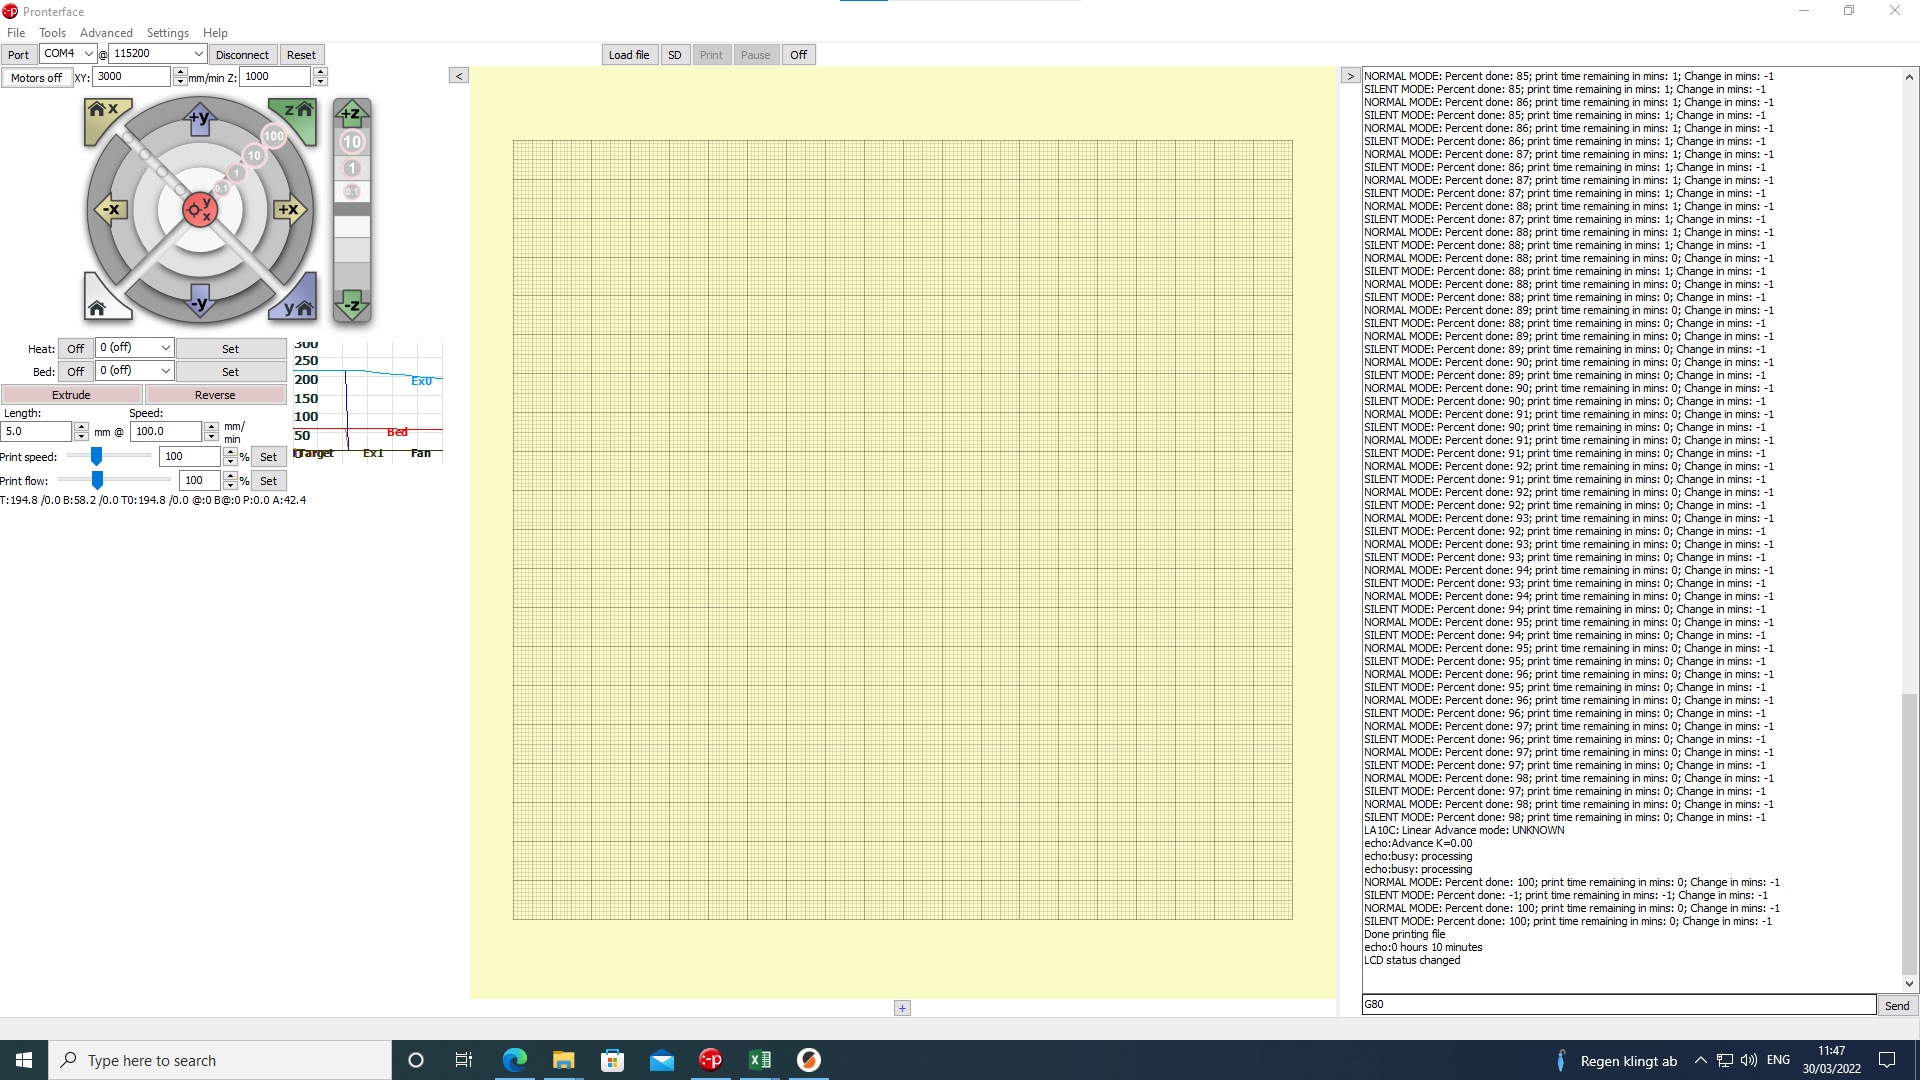
\includegraphics[width=350px]{./images/printrun.png}}
	\caption{Programm PrintRun}
	\label{printrun}
	\end{figure}

In Abbildung \ref*{printrun} ist die Bedienoberfläche des Programms zu sehen, womit man unter anderem den Druckkopf oder die Bodenplatten bewegen kann. Nach eingeben des G80 Befehls begann der Drucker mit Hilfe des Druckkopfes due Bodenplatte abzumessen, und nach Erfolgreicher Beendigung konnte man mit G81 die gemessenen Werte ausgeben lassen.

Im Anschluss wurden die Raupe sowie der Quader mit in Tabelle \ref*{tab:z-offset} aufgelisteten z-offset Werten gedruckt. Jedes gedruckte Objekt wurde dann in der Breite an fünf Stellen ausgemessen. Leider bot der Drucker nicht die vorgegebenen Abweichungen nicht an, weswegen die Ist-Werte leicht daneben liegen.  

\bgroup
\def\arraystretch{1.6}%
\begin{table}[H]
\centering
\label{tab:z-offset}
\begin{tabular}{|c|c|}
\hline
z-offset Soll {[}mm{]} & z-offset Ist {[}mm{]} \\ \hline
-0,006                 & -0,008                \\ \hline
-0,003                 & -0,003                \\ \hline
+0,003                 & +0,003                \\ \hline
+0,006                 & +0,005                \\ \hline
\end{tabular}
\caption{Z-offset Werte Ist und Soll}
\end{table}
\egroup

\section[Auswertung und Analyse]{Auswertung und Analyse}
Die Druckbettnivellierung ergab die in Tabelle \ref*{tab:druckbett1} zu sehende Werte. Da hier jedoch nicht ersichtlich war, welche Ecke welcher Position in der Matrix zuzuordnen war, wurde für einen weiteren Messlauf in die vordere linke Ecke ein Stück Papier untergelegt, was zu der in Tabelle \ref*{tab:druckbett2} aufgelisteten Werte führt. Man erkennt deutlich die gestiegenen Werte, und zudem wurde klar, dass die vordere linke Ecke des Bettes die untere linke Ecke der Matrix abgebildet wird. 

\begin{table}[H]
\centering
\caption{Z-Offset Niveau Werte des Druckbetts}
\label{tab:druckbett1}
\begin{tabular}{|l|l|l|l|l|l|l|}
\hline
-0,18917 & -0,16833 & -0,14333 & -0,11917 & -0,14667 & -0,19833 & -0,295   \\ \hline
-0,14167 & -0,10417 & -0,09333 & -0,14917 & -0,14167 & -0,18083 & -0,2825  \\ \hline
-0,08    & -0,045   & -0,045   & -0,08333 & -0,09583 & -0,15417 & -0,265   \\ \hline
-0,03833 & -0,0375  & -0,03333 & -0,04333 & -0,085   & -0,16167 & -0,26333 \\ \hline
0,05417  & 0,06     & 0,03667  & -0,00833 & -0,03917 & -0,10833 & -0,26083 \\ \hline
0,105    & 0,095    & 0,06833  & 0,0125   & -0,03333 & -0,09083 & -0,24667 \\ \hline
0,1725   & 0,14167  & 0,12583  & 0,04917  & 0,01     & -0,08583 & -0,19333 \\ \hline
\end{tabular}
\end{table}

\begin{table}[H]
\centering
\caption{Z-Offset Werte des mit Papier unterlegtem Druckbetts}
\label{tab:druckbett2}
\begin{tabular}{|l|l|l|l|l|l|l|}
\hline
-0,20167 & -0,1925  & -0,16417 & -0,14167 & -0,1725  & -0,235   & -0,32083 \\ \hline
-0,1575  & -0,12333 & -0,11417 & -0,16333 & -0,16    & -0,20417 & -0,29583 \\ \hline
-0,09583 & -0,06167 & -0,06417 & -0,10208 & -0,11833 & -0,16167 & -0,27833 \\ \hline
-0,04583 & -0,045   & -0,055   & -0,0625  & -0,10854 & -0,18833 & -0,27917 \\ \hline
0,07917  & 0,0825   & 0,02     & -0,02854 & -0,065   & -0,12667 & -0,2875  \\ \hline
0,4      & 0,23333  & 0,07833  & -0,00667 & -0,055   & -0,12417 & -0,25917 \\ \hline
0,65083  & 0,24667  & 0,10167  & 0,01667  & -0,02333 & -0,12583 & -0,21    \\ \hline
\end{tabular}
\end{table}

Visualisiert in Abbildung \ref*{fig:druckbett3d} erkennt man die Schieflage des Druckbetts. Dank der integrierten Funktion des Druckers, diese vor jedem Druck zu messen und auszugleichen, ist das keine Sache die zu beachten ist.

\begin{figure}[H]
\centerline{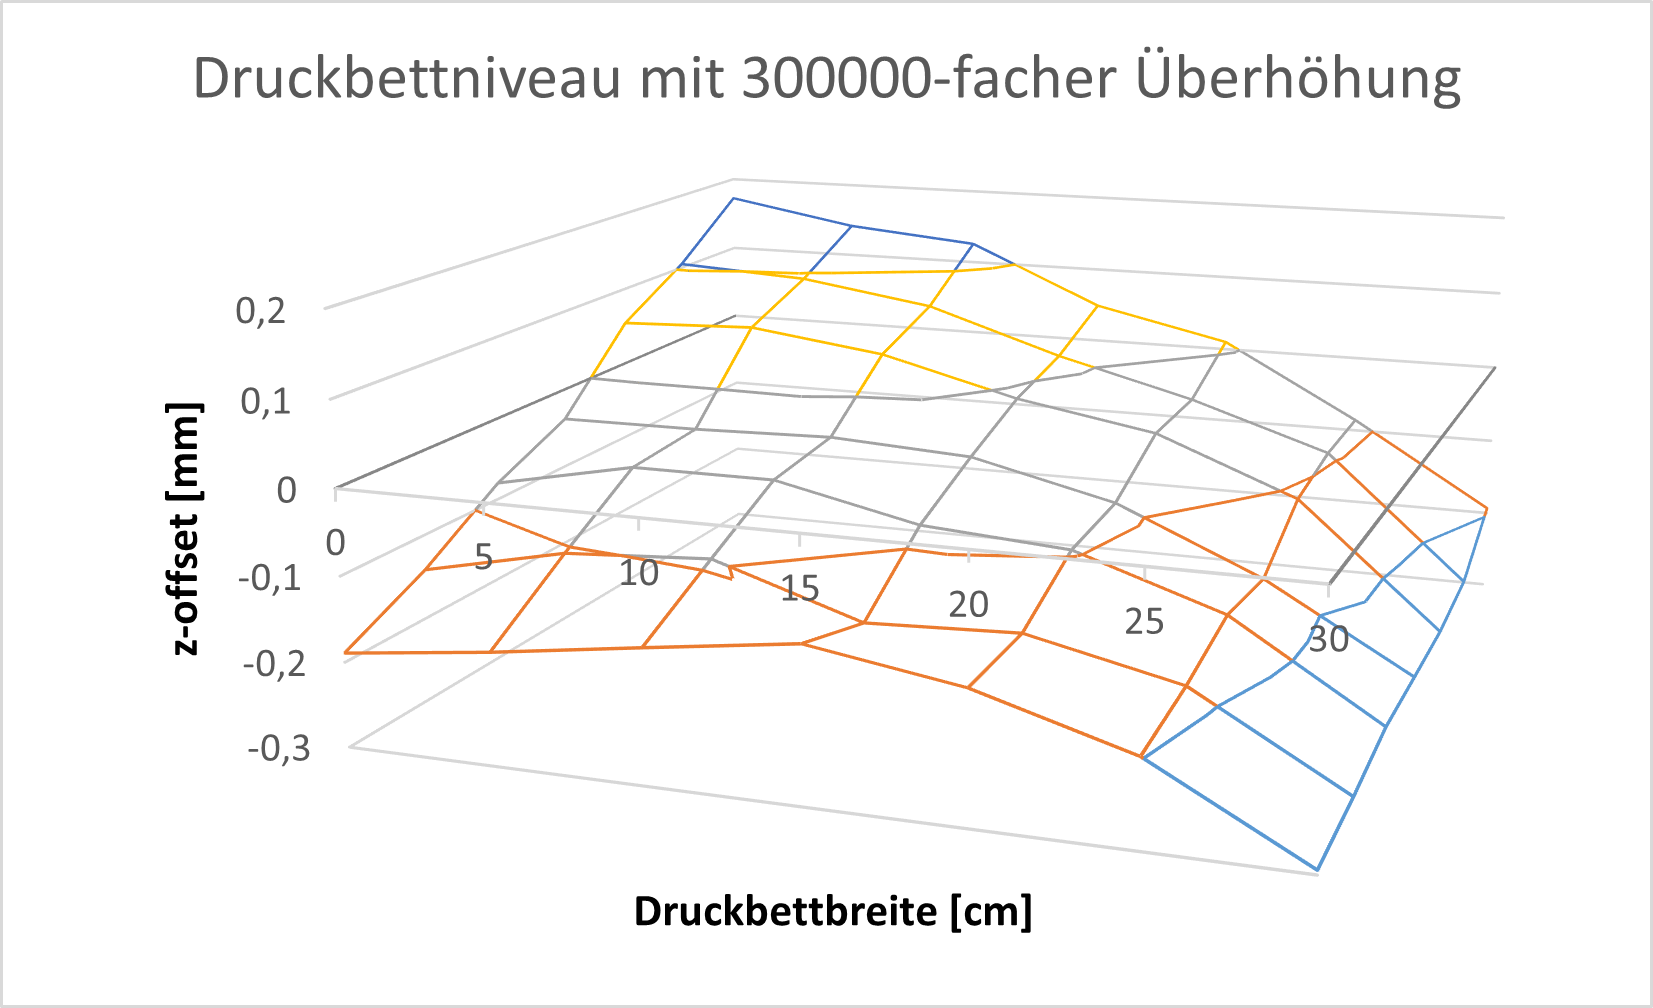
\includegraphics[width=350px]{./images/diagramm.png}}
\caption{3D Visualisierung des Druckbetts}
\label{fig:druckbett3d}
\end{figure}


Überhöhung


\newpage
\begin{thebibliography}{999}
\bibitem{Quelle} Versuchsanleitung zu (Abgerufen am 23.03.2022) 
\end{thebibliography}

% Für Dokumente mit mehr Referenzen empfiehlt es sich, auf eine separate .bib -Datei umzusteigen, die alle Referenzen enthält. Diese Referenzen können bei den meisten wissenschaftlichen Publikationen direkt über "BibTex-Export" oder ähnliches heruntergeladen werden. Anstelle von \begin{thebibliography}...\bibitem{}..\bibitem{}..\end{thebibliography} muss dann lediglich \bibliography{Dateiname.bib} eingebunden werden.

%\section{Anhang}
%\includepdf[pages=-]{Dateiname.pdf}


\end{document}